%%%%%%%%%%%%%%%%%%%%%%%%%%%%%%%%%%%%%%%%%%%%%%%%%%%%%%%%%%%%%%%%%%%%%%%%%%%%%%%%
%2345678901234567890123456789012345678901234567890123456789012345678901234567890
%        1         2         3         4         5         6         7         8

\documentclass[letterpaper, 10 pt, conference]{ieeeconf}  % Comment this line out if you need a4paper

%\documentclass[a4paper, 10pt, conference]{ieeeconf}      % Use this line for a4 paper

\IEEEoverridecommandlockouts                              % This command is only needed if 
                                                          % you want to use the \thanks command

\overrideIEEEmargins                                      % Needed to meet printer requirements.

\usepackage{epsfig} %% for loading postscript figures
\usepackage{mathtools}   % loads �amsmath�
\usepackage{amssymb,amsmath}
\usepackage{amsfonts}
\usepackage{multirow}
%\usepackage{natbib}
\usepackage{relsize}
\usepackage{graphicx}
\usepackage{color}
\usepackage{comment}

% See the \addtolength command later in the file to balance the column lengths
% on the last page of the document

% The following packages can be found on http:\\www.ctan.org
%\usepackage{graphics} % for pdf, bitmapped graphics files
%\usepackage{epsfig} % for postscript graphics files
%\usepackage{mathptmx} % assumes new font selection scheme installed
%\usepackage{times} % assumes new font selection scheme installed
%\usepackage{amsmath} % assumes amsmath package installed
%\usepackage{amssymb}  % assumes amsmath package installed


\title{\LARGE \bf
Robot Assisted Ultrasound Guided Catheter Tracking
}

\begin{comment}
\author{Albert Author$^{1}$ and Bernard D. Researcher$^{2}$% <-this % stops a space
\thanks{*This work was not supported by any organization}% <-this % stops a space
\thanks{$^{1}$Albert Author is with Faculty of Electrical Engineering, Mathematics and Computer Science,
        University of Twente, 7500 AE Enschede, The Netherlands
        {\tt\small albert.author@papercept.net}}%
\thanks{$^{2}$Bernard D. Researcheris with the Department of Electrical Engineering, Wright State University,
        Dayton, OH 45435, USA
        {\tt\small b.d.researcher@ieee.org}}%
}
\end{comment}

\begin{document}



\maketitle
\thispagestyle{empty}
\pagestyle{empty}


%%%%%%%%%%%%%%%%%%%%%%%%%%%%%%%%%%%%%%%%%%%%%%%%%%%%%%%%%%%%%%%%%%%%%%%%%%%%%%%%
\begin{abstract}

\end{abstract}


%%%%%%%%%%%%%%%%%%%%%%%%%%%%%%%%%%%%%%%%%%%%%%%%%%%%%%%%%%%%%%%%%%%%%%%%%%%%%%%%
\section{INTRODUCTION}


\section{PLATFORM SETUP}
\subsection{Early Stage : Matlab ( Experiment Only )}
\begin{itemize}
\item Implementation of simple position control
\end{itemize}

\subsection{Middle Stage : C-API ( Experiment Only )}
\begin{itemize}
\item Install C-API on a public desktop/laptop
\item Transfer the control law from Matlab/ROS to C-API if necessary
\end{itemize}


\subsection{Final Stage : ROS ( Experiment and Simulation )} 
Environment Setup:
\begin{itemize}
\item Insert 3D model of the phantom
\item Insert 3D model of the container
\item Insert 3D model of the ultrasound sensor and its holder, and attach them to the end-effector of UR5
\item Specify the pose for both the phantom and the container
\item Specify the starting configuration of UR5
\item (Future) Include the force sensor 3D model  
\end{itemize}


\subsection{Basic Functionality Test}
\begin{itemize}
\item Forward kinematics and inverse kinematics
\item Joint limit specification
\item Implementation of the control law
\item (Future) Force/torque feedback
\end{itemize}


\section{HARDWARE COMMUNICATION}
\begin{figure}[h]
\includegraphics[scale=0.04]{UR5_phantom.png}
\centering
\end{figure}

\begin{figure}[h]
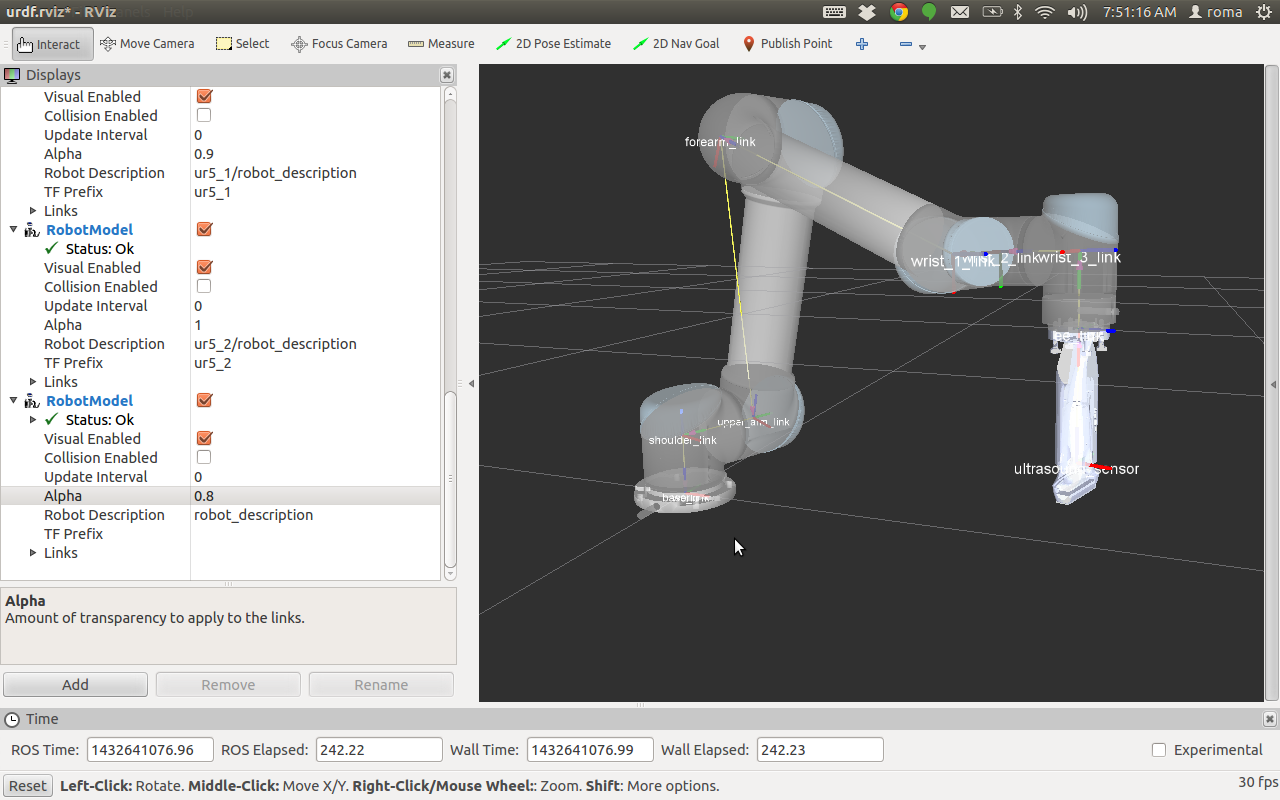
\includegraphics[scale=0.2]{UR5_phantom_ROS_simulator.png}
\centering
\end{figure}

\begin{figure}[h]
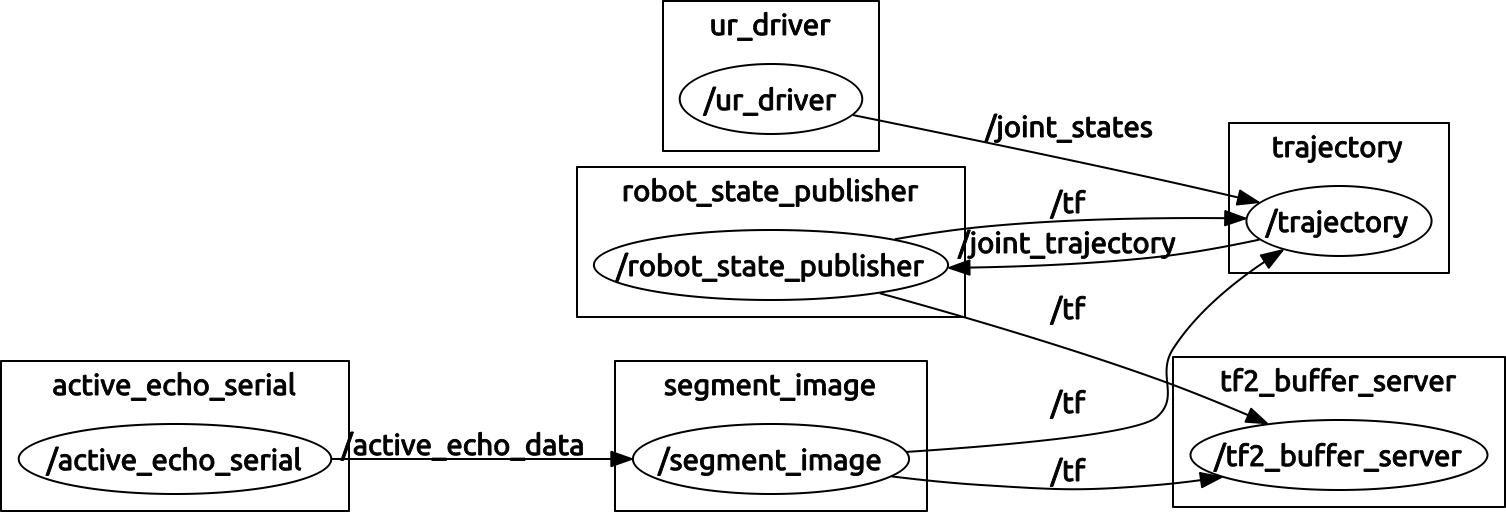
\includegraphics[scale=0.2]{UR5_ultrasound_ROS_system.png}
\centering
\end{figure}



\begin{itemize}
\item Computer and UR Controller Box
\begin{itemize}
\item Matlab - Windows - PC - Controller Box  (Done by Fereshteh )
\item C-API - Windows - PC - Controller Box ( Done by Tutken )
\item ur-driver - ROS - Linux - PC - Controller Box ( To be tested ) 
\end{itemize}

\item Computer and  [Ultrasound Sensor + Active echo ]

\item Computer and Force Sensor
		Questions: sensor specifications, force feedback model 
\item Computer and Catheter 
	PC - Controller Box - Catheter : for robot assisted catheter steering
\end{itemize}


\section{Control Law}
Input
\begin{itemize}
\item Intensity information ( from active echo ) 
\item  2D-Position of the catheter ( from active echo )
\end{itemize}

Output
\begin{itemize}
\item Pose of the ultrasound sensor (Early Stage)
\item Twist of the ultrasound sensor (Final Stage)
\end{itemize}

Workspace Constraint
		Bounding box of the workspace which is defined by the sizes of the container and phantom
	
Velocity Constraint
\begin{itemize}
\item $Vz : 0$
\item $|Vx| < const$
\item $|Vy| < const$
\end{itemize}

Force/torque Constraint (Future)
\begin{itemize}
\item $1. 0 < |Fz| < const$
\end{itemize}


Feedback 
\begin{itemize}
\item Ultrasound image  Active echo information
\item Force  Torque
\end{itemize}


Algorithm
\begin{itemize}
\item Intensity/Position feedback algorithm 
\item Force/Torque feedback algorithm
\item Moving direction feedback given known start and end position, and bounding box of the workspace
\end{itemize}


\section{Calibration}
\begin{itemize}
\item Step 1 Generate calibration script for UR5 with a phantom (AX = XB problem)
\item Step 2 Determine the appropriate relative distance between the ultrasound sensor and the phantom:

\end{itemize}


\section{Experiment Setup Up}
\begin{itemize}
\item Best fluid for active echo (milk or fluids other than water)
\item Fixed position for the container and the phantom
\item Proper container to operate the catheter
\item Install the active echo on the tip of the catheter 
\end{itemize}

\section{CONCLUSIONS}

\addtolength{\textheight}{-12cm}   % This command serves to balance the column lengths
                                  % on the last page of the document manually. It shortens
                                  % the textheight of the last page by a suitable amount.
                                  % This command does not take effect until the next page
                                  % so it should come on the page before the last. Make
                                  % sure that you do not shorten the textheight too much.

%%%%%%%%%%%%%%%%%%%%%%%%%%%%%%%%%%%%%%%%%%%%%%%%%%%%%%%%%%%%%%%%%%%%%%%%%%%%%%%%



%%%%%%%%%%%%%%%%%%%%%%%%%%%%%%%%%%%%%%%%%%%%%%%%%%%%%%%%%%%%%%%%%%%%%%%%%%%%%%%%



%%%%%%%%%%%%%%%%%%%%%%%%%%%%%%%%%%%%%%%%%%%%%%%%%%%%%%%%%%%%%%%%%%%%%%%%%%%%%%%%
\section*{APPENDIX}


\section*{ACKNOWLEDGMENT}



%%%%%%%%%%%%%%%%%%%%%%%%%%%%%%%%%%%%%%%%%%%%%%%%%%%%%%%%%%%%%%%%%%%%%%%%%%%%%%%%




\end{document}
